\documentclass{article}

\usepackage[margin=3cm]{geometry}
\usepackage{fontspec}
    \setsansfont{Linux Biolinum O}
\usepackage{polyglossia}
    \setmainlanguage{english}
\usepackage{sectsty}
    \sectionfont{\normalfont\sffamily\bfseries\color{blue!40!black}}
    \subsectionfont{\normalfont\sffamily\bfseries\color{blue!30!black}}
\usepackage{float}
\usepackage{booktabs}
\usepackage{subcaption}
\usepackage{graphicx}
\usepackage{xcolor}
\usepackage{listings}
    \lstset{language=c,
	basicstyle=\footnotesize\ttfamily,
	breaklines=true,
	framextopmargin=50pt,
	frame=bottomline,
	backgroundcolor=\color{white!86!black},
	commentstyle=\color{blue},
	keywordstyle=\color{red},
	stringstyle=\color{orange!80!black}}
\usepackage{tikz}

\title{\textsf{\color{blue!40!black}2. Übung IBN}}
\author{Maurice Donner \and Ise Glade}

\begin{document}
\maketitle

\section*{Aufgabe 1}
The script can be found in the \texttt{.zip} folder and is called \texttt{order.sh}.
The folder also contains a directory with some test images, which have different
timestamps. Use \texttt{./order.sh -h} to print the help information.

\section*{Aufgabe 2}
\begin{itemize}
    \item[a.] The \texttt{files\_struct} contains pointers to up to \textbf{256}
	\texttt{file} data structures. In todays systems, the maximum number of
	files a process is able to use is 1048576 (as on Kernel version 5.10.0).
	Other sources give different numbers which depend on the Kernel version.
	\\ This limit can however be changed by simply writing to the file\\
	\texttt{/proc/sys/fs/file-max}.
    \item[b.] The struct \texttt{files\_struct} is referenced on \textbf{line 1073}.
	Its source code looks like the following:
\begin{lstlisting}
struct files_struct {
        atomic_t    count;              /* structure's usage count */
        spinlock_t  file_lock;          /* lock protecting this structure */
        int         max_fds;            /* maximum number of file objects */
        int         max_fdset;          /* maximum number of file descriptors */
        int         next_fd;            /* next file descriptor number */
        struct file **fd;               /* array of all file objects */
        fd_set      *close_on_exec;     /* file descriptors to close on exec() */
        fd_set      *open_fds;           /* pointer to open file descriptors */
        fd_set      close_on_exec_init; /* initial files to close on exec() */
        fd_set      open_fds_init;      /* initial set of file descriptors */
        struct file *fd_array[NR_OPEN_DEFAULT]; /* default array of file objects */
};
\end{lstlisting}
The \texttt{files\_struct} contains all per-process information about open files
and file descriptors.
\end{itemize}

\newpage

\section*{Aufgabe 3}
This program creates exactly \( 2 ^{n} \) processes, where \( n \) is the
command line argument. For \( n = 10 \) this is equal to 1024 processes.\\
The reason for this is that with each new iteration, the variable
\texttt{i} is inherited by the child process, leading to a tree-like
structure that is visualised below
\begin{figure}[H]
    \centering
    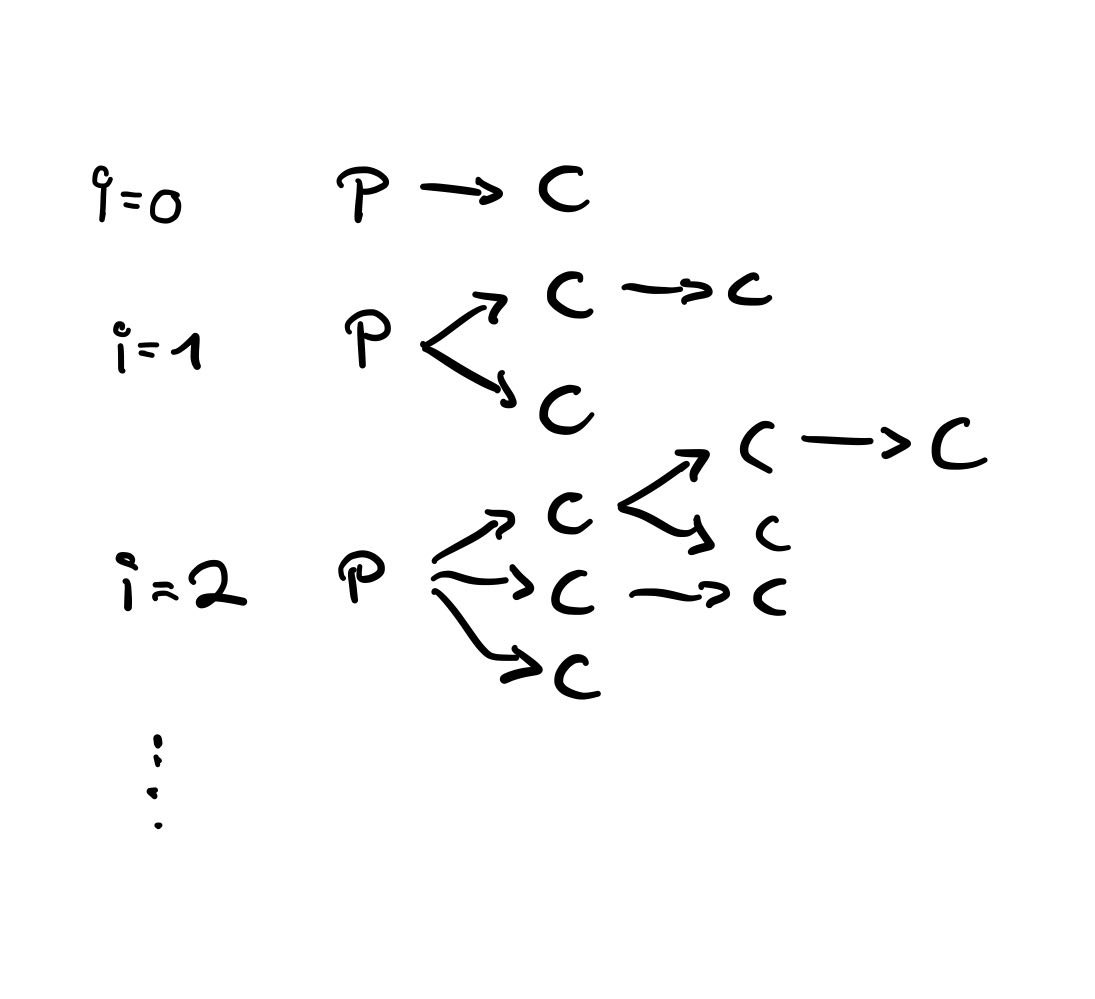
\includegraphics[width=.5\textwidth]{Fork.jpg}
\end{figure}
\section*{Aufgabe 4}
\textbf{a.} The \texttt{bash} command \texttt{bs} gives a snapshot of the currently
running processes. Options such as -aux lets the user get a full list of all
processes, even those not associated with a terminal.
\textbf{b.} There exist five states of processes in Linux:
\begin{itemize}
\item Running or Runnable (R)
\item Uninterruptible Sleep (D) \\ This is the \textit{waiting-} state 
    from the lecture. The process might be waiting for I/O, or other resources.
\item Interruptable Sleep (S) \\
    Similar to \texttt{D}, but with the additional option to be woken up by a
    signal.
\item Stopped (T)
    This is the interrupted state, where a process has recieved the
    \texttt{SIGSTOP} signal, and can be turned back into the runnable
    state by recieving a \texttt{SIGCONT} signal.
\item Zombie (Z)
    This state is usually used by child processes, that have finished their
    execution, and are waiting for the parent process to terminate them.
\end{itemize}
\newpage
\section*{Aufgabe 5}
\textbf{a.} All we need to do to synchronize the threads is to join each
thread after it finished running:
\begin{figure}[H]
    \centering
    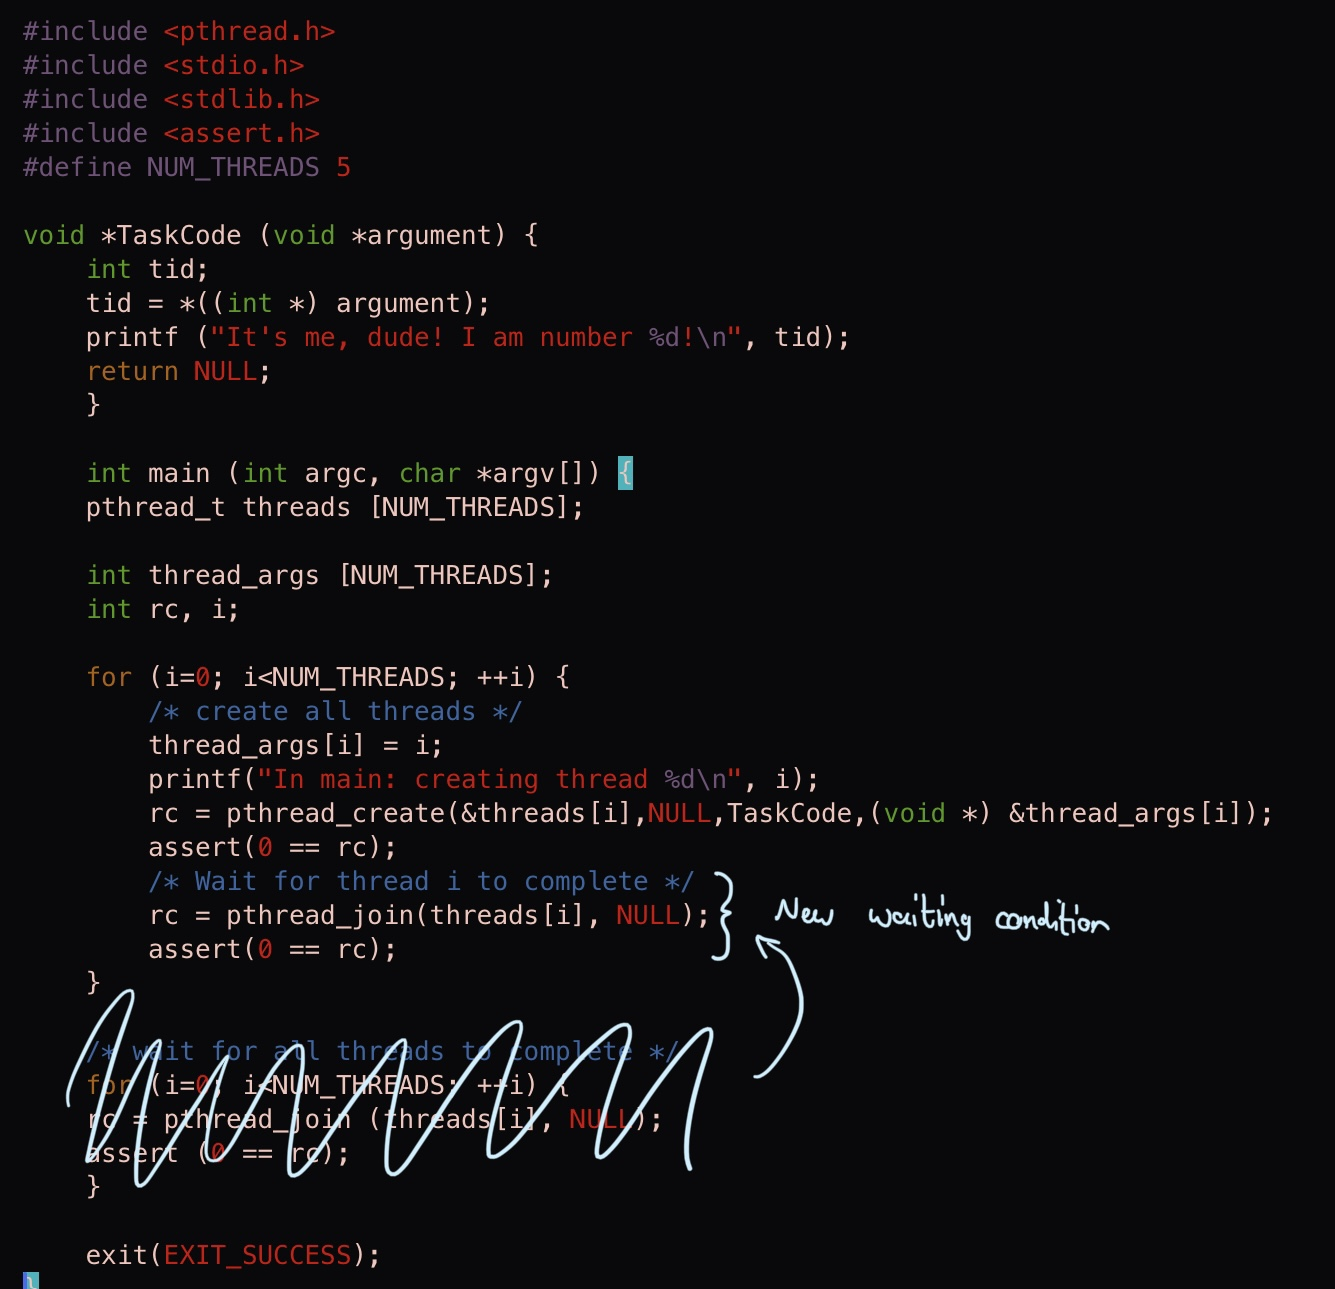
\includegraphics[width=.7\textwidth]{Threads.jpg}
\end{figure}
\noindent Note however, that this completely negates the purpose of creating the threads
in the first place! The standard output will look like this:
\begin{lstlisting}
In main: creating thread 0
It's me, dude! I am number 0!
In main: creating thread 1
It's me, dude! I am number 1!
In main: creating thread 2
It's me, dude! I am number 2!
In main: creating thread 3
It's me, dude! I am number 3!
In main: creating thread 4
It's me, dude! I am number 4!
\end{lstlisting}
\textbf{b.} For \texttt{NUM\_THREADS} \( > 200000 \) the execution of
the program starts taking longer than 9 seconds.
\textbf{c.} Running \texttt{TaskCode} in a single sequential program
200000 times takes about \( 0.6 \)s.\\
One of the reasons for the drastic decrease in runtime is the printing to
stdout. Printing, that a thread has been created and printing its
thread id, already slows down the program by approximately a factor of 2
(on the used system). However, this still doesn't explain the 5 seconds
the program still needs, which might be spent creating and terminating threads.
Creating threads could therefore be a relatively slow process, but only if
the runtime of the task they perform is in the order of thread creation itself.\\
\newpage
\noindent The system used for this task is the following:
\begin{lstlisting}
OS: Debian GNU/Linux 11 (bullseye) x86_64 
Host: 42915CG ThinkPad X220 
Kernel: 5.10.0-9-amd64 
Uptime: 18 days, 10 hours, 15 mins 
Packages: 2882 (dpkg) 
Shell: bash 5.1.4 
Resolution: 1920x1080 
Terminal: /dev/pts/5 
CPU: Intel i5-2520M (4) @ 3.200GHz 
GPU: Intel 2nd Generation Core Processor Family 
Memory: 2780MiB / 7839MiB
\end{lstlisting}
\section*{Aufgabe 6}
\begin{itemize}
    \item The first level is rather easy, as the global variable \texttt{flag}
	is set true, and both threads can enter the critical region immediately.
    \item The second level can be solved by first increasing the right counter
	three times (three-headed dragon), enter
	the critical region, and then the left counter another two
	times (five-headed dragon). Since it is the same counter variable that
	is changed, both threads can enter the critical region.
    \item The third level can be solved, by expanding the operation of increasing
	the variable \texttt{first}. If both threads store its value at the same
	time into the variable \texttt{temp}, it will never be increased above 1,
	therefore fulfilling the condition and breaking the program.
\end{itemize}
\section*{Aufgabe 7}
\textbf{a.}
\begin{itemize}
    \item \texttt{TSL}: The thread copies the lock value and sets it to something \( 
	    \neq 0  \).
    \item \texttt{CMP} It then checks if the value copied from lock is 0. If no, it
       may proceed.
   \item \texttt{RET} It then leaves the routine \texttt{enter\_region} and
      enters the critical area. 
\end{itemize}
\textbf{b.} 
\begin{itemize}
    \item \texttt{TSL}: The thread copies the lock value and sets it to something \( 
	    \neq 0  \).
    \item \texttt{CMP} It then checks if the value copied from lock is 0.
	If yes, another thread previously requested the lock, and our first
	thread has to wait. It enters the wait loop.
	\item \texttt{JNE} The thread jumps back to the start of
	    \texttt{enter\_region} and starts over from step 1: \texttt{TSL}. 
	\item This happens another time, before the value copied from the
	   register is 0. The third time, it then may proceed. 
       \item \texttt{RET} The thread leaves the routine \texttt{enter\_region}
	   and enters the critical area.
\end{itemize}
Below, the processes are quickly sketched:
\begin{figure}[H]
    \centering
    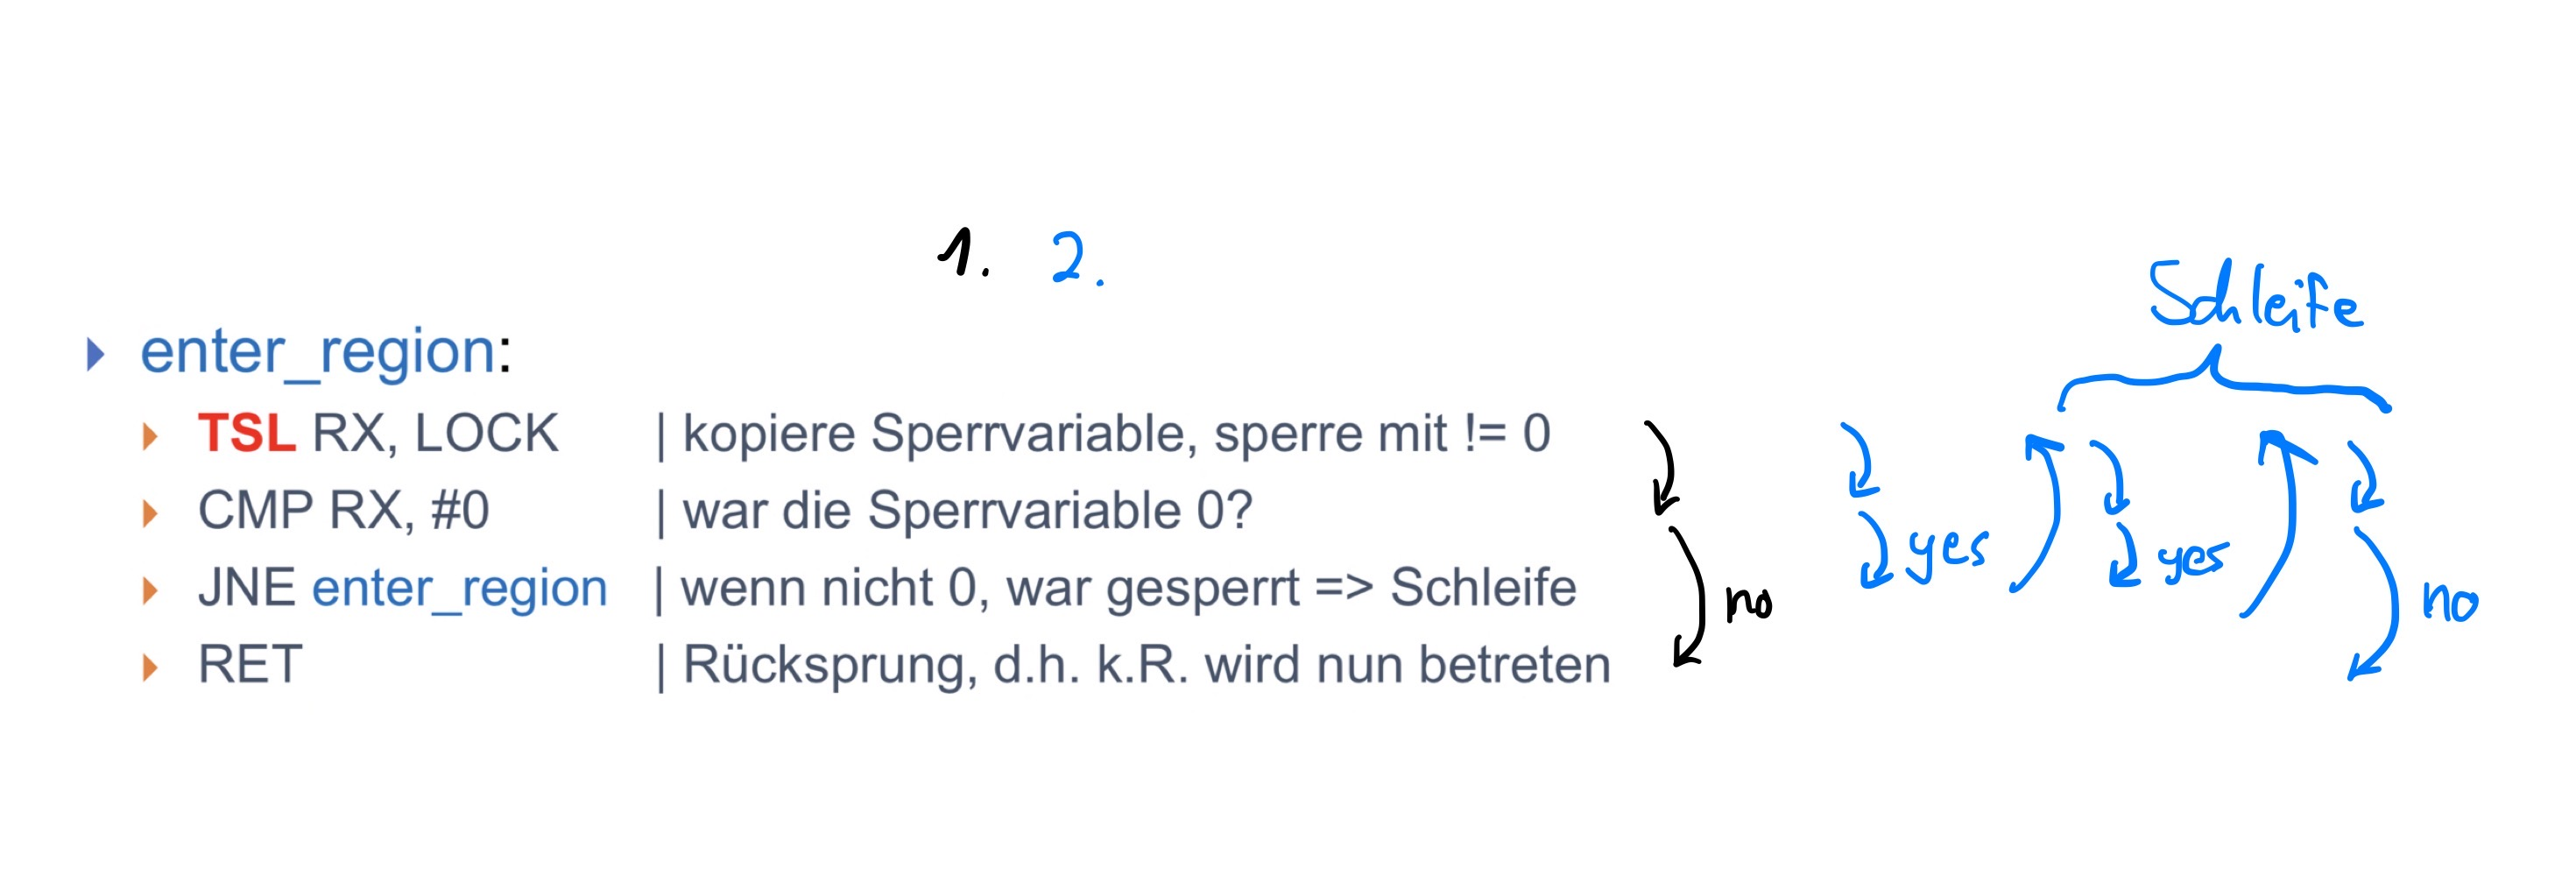
\includegraphics[width=.8\textwidth]{Sketch.jpg}
\end{figure}
\end{document}
